\documentclass{article}
\usepackage{graphicx}
\usepackage{amsmath}
\usepackage[parfill]{parskip}
\usepackage{hyperref}
\graphicspath{ {./figures/} }

\usepackage{listings}
\usepackage{xcolor}

\definecolor{codegreen}{rgb}{0,0.6,0}
\definecolor{codegray}{rgb}{0.5,0.5,0.5}
\definecolor{codepurple}{rgb}{0.58,0,0.82}
\definecolor{backcolour}{rgb}{0.95,0.95,0.92}

\lstdefinestyle{mystyle}{
    backgroundcolor=\color{backcolour},   
    commentstyle=\color{codegreen},
    keywordstyle=\color{magenta},
    numberstyle=\tiny\color{codegray},
    stringstyle=\color{codepurple},
    basicstyle=\ttfamily\footnotesize,
    breakatwhitespace=false,         
    breaklines=true,                 
    captionpos=b,                    
    keepspaces=true,                 
    numbers=left,                    
    numbersep=5pt,                  
    showspaces=false,                
    showstringspaces=false,
    showtabs=false,                  
    tabsize=2
}

\lstset{style=mystyle}

\title{COMP.SEC.220 Security Protocol\footnote{github --- \url{https://github.com/ancuongnguyen07/SecurityProtocol}}}
\author{Cuong Nguyen --- LAB 3}
\date{09/09/2022}

\begin{document}
    
\maketitle

\section*{Exercise 1}
%
\begin{itemize}
    \item Alice (A): Signer --- Sender
    \item Bob (B): Verifier --- Recipient
    \item \emph{m}: message
    \item \emph{h}: hash function
    \item \emph{E}: encrytion
    \item \emph{D}: decryption
    \item \emph{pk}: public key
    \item \emph{sk}: secret key
\end{itemize}

\textbf{Verification process:}\\
Firstly, Bob recieves a signed hash-digest of message \(E_{sk_{A}}
(h(m))\), then he must decrypt it using the Alice's public key (\(
D_{pk_{A}}(E_{sk_{A}}(h(m)))\)) to get the hash-digest of the original
message --- called \emph{hashA}. Secondly, Bob need to calculate the
hash-digest of the plain message he recieved --- called \emph{hashB}.
Finally, comparing \emph{hashA} and \emph{hashB}, if they are equal then
the message is authentic. 

\begin{figure}[hpt]
    \centering
    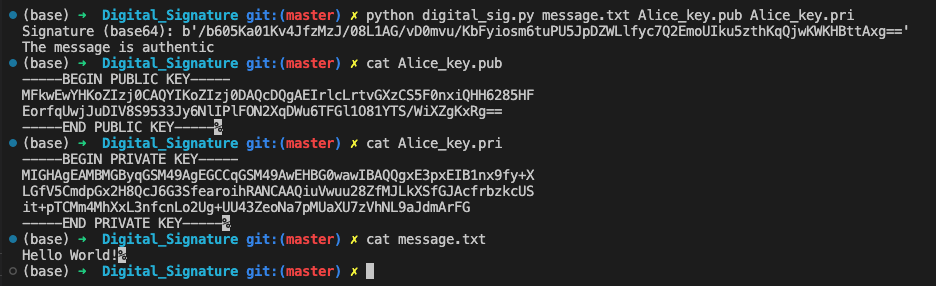
\includegraphics[width=\textwidth,height=35mm,keepaspectratio]{ds.png}
    \caption{Commands of verifying a signature}
    \label{fig:ds}
\end{figure}

\section*{Exercise 2 + 3}
%
Below is the Shell script automate generating key pairs, CSR, Certificate
\lstinputlisting[language=bash, caption=Automated Shell Script]{python/CA/ca.sh}

%
\begin{figure}[hpt]
    \centering
    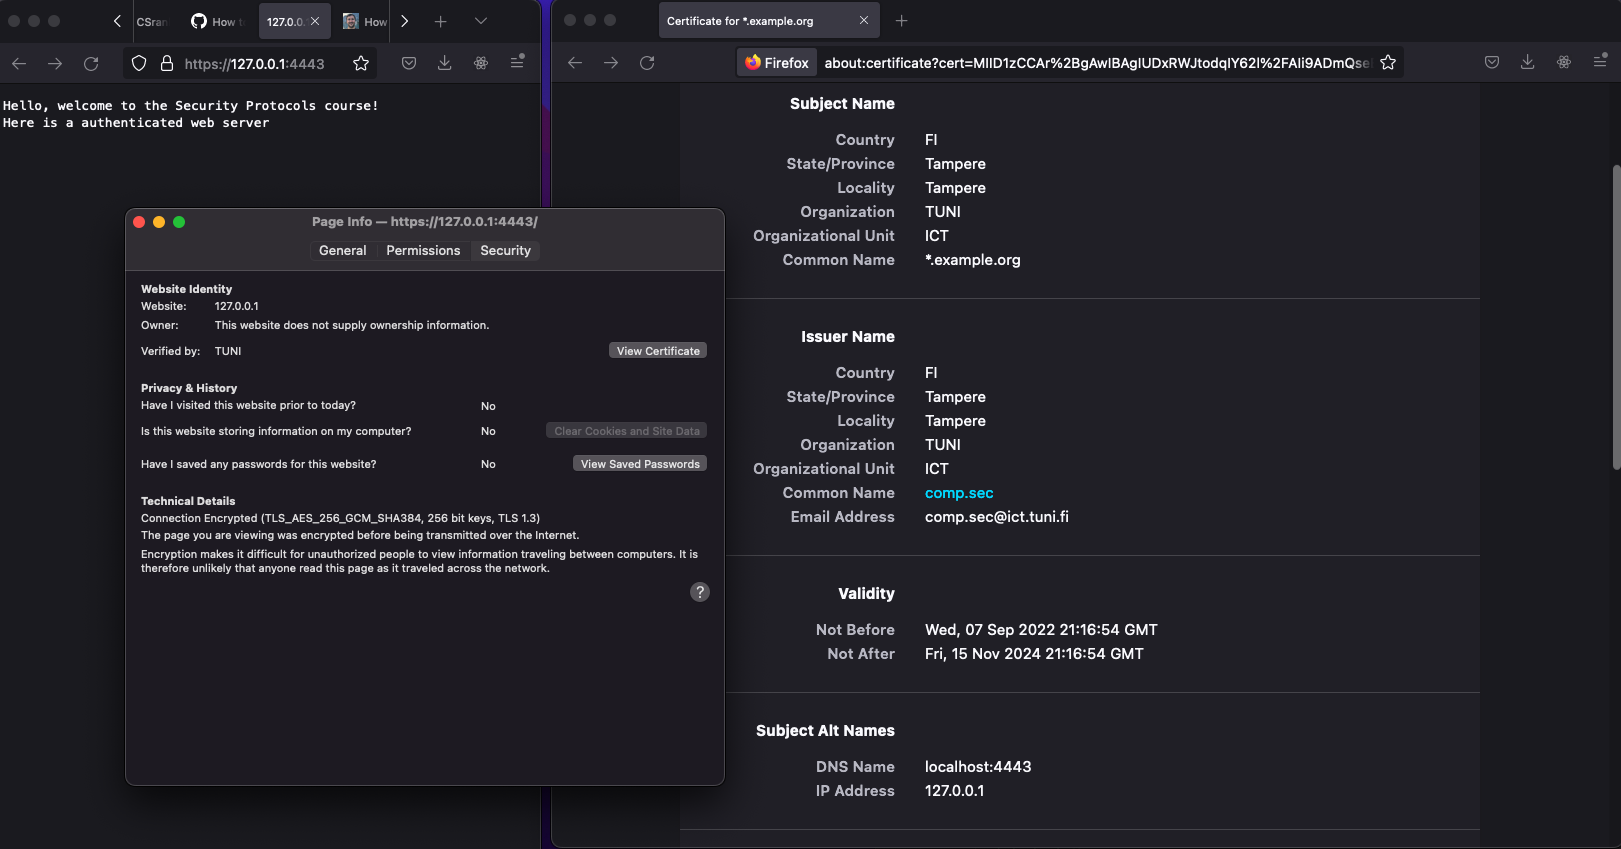
\includegraphics[width=\textwidth,height=\textheight,keepaspectratio]{cert.png}
    \caption{A web server with certificate information displayed}
    \label{fig:cert}
\end{figure}

\section*{Exercise 4}
%
In order to send a encrypted e-mail message to a recipient, the sender must have
the public key of the intended recipient to encrypt the message and deliver it.
Then the recipient can decrypt the message by using his/her private key.

\end{document}